\documentclass[a4paper,8pt,french,fleqn]{article}
%Packages:

%Langages:
\usepackage[french]{babel}
\usepackage{lmodern}
\usepackage[T1]{fontenc}
\usepackage[utf8]{inputenc}
%AMS maths
\usepackage{amsmath, amssymb, amsfonts}

%Mise en page
\usepackage[top=2cm, right=2cm, bottom=2cm, left=2cm]{geometry}
\usepackage{fancyhdr}
\usepackage{enumerate}
\usepackage{color}
%Définition des macros
\usepackage{amsthm}

%Figures
\usepackage{tikz}
\usepackage{graphicx}
\usepackage{wrapfig}
\usepackage[french, vlined, lined, linesnumbered, boxed]{algorithm2e}
%Symboles mathématiques
\usepackage{latexsym}
\usepackage{sidecap}
\usepackage{bm}

\begin{document}

\section{Pendule à N maillons}

On a commencé dans cette partie par étudier le cas d'un pendule simple sans d'approximation pour les amplitudes.
Pour ce système, on peut se limiter à la position du maillon car l’état du pendule peut être déduit par le maillon. Et puisque le seul paramètre qui change est le degrés car on suppose que la longueur $\mathcal{l}$  fixe tout au long du mouvement (pas d'élasticité) donc on peut se limiter au degré $\theta$.\\

En utilisant le théorème d’énergie mécanique et en utilisant l'équation du bilan de force, on peut arriver à avoir l'équation:$ \dot{\theta^2} + 2 \omega_0^2 ( \cos\theta_0 - \cos\theta) = 0$. Cette équation peut être approximé pour les grandes amplitudes par  $T(\theta_0) = T_0 ( 1 + \frac{\theta_0^2}{16} )$: \textbf{Approximation de Borda}.\\\\
On utilise donc cette équation et on trace les fréquences dans l'intervalle $[-\pi , \pi]$ :
\begin{figure}[h]
\centering
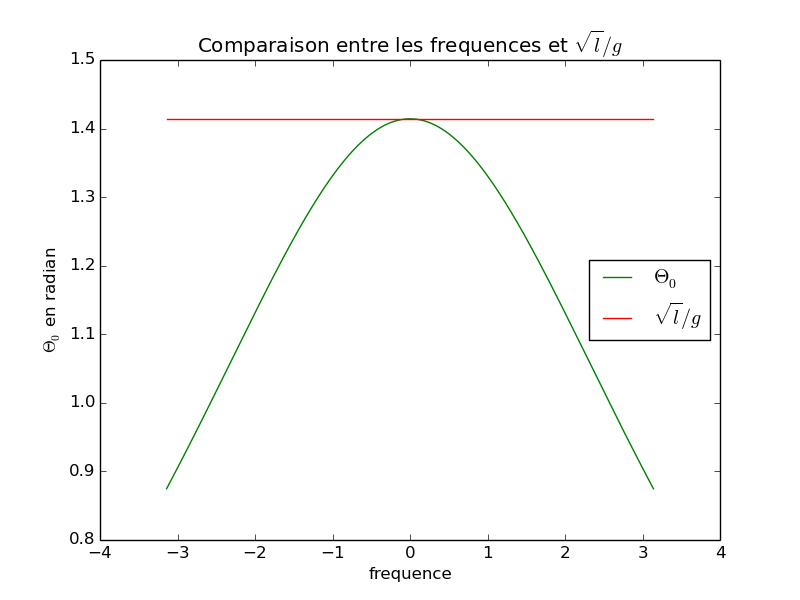
\includegraphics[scale=0.4]{images/un_maillon}
\caption{Comparaison entre la fréquence et $\sqrt{l}/g$}
\end{figure}  
On remarque que lorsque les oscillations deviennent très petites, c-à-d convergent vers 0, la fréquence converge vers $\sqrt{l}/g$.\\
On a ensuite essayé d'étudier le système à deux maillons qui est un système dit chaotique.\\
En remarquant que vu qu'on néglige encore l’élasticité du fil, on peut ainsi modéliser notre système par deux paramètres {$\theta_1$ et $\theta_2$}. On peut justifier cette modélisation par le fait de pouvoir obtenir toutes les positions avec ses deux paramètres en utilisant le système suivant:\\
%\begin{figure}[h]
%\begin{center}
\begin{equation}
 \begin{cases}
 x1 =  L_1 \times  \sin{\theta_1} \\
 y1 = - L_1 \times \cos{\theta_1} \\
 x2 = x1 + L_2 \sin{\theta_2} \\
 y2 = y1 - L_2 \cos{\theta_2} 
\end{cases}
\end{equation}
%\caption{Position de deux maillons en fonction de $\theta_1$ et $\theta_2$}
%\end{center}
%\end{figure}
Ainsi, le problème se limite à la recherche des angles. Après une simplifications des equations obtenue avec le bilan de forces et le bilans d’Énergie mécanique, on arrive au système suivant:\\\\
\begin{equation}
\begin{cases}
 \theta_1' = \omega_1 \\\theta_2'= \omega_2
 \\
\omega_1' = \frac{-g(2 m_1 + m_2)\sin{\theta_1} - gm_2 sin(\theta_1- 2\theta_2)- 2\sin{\theta1 - \theta_2m2(\omega_{2}^2 L_2 + \omega_{1}^2 L_1\cos(\theta_1 - \theta_2))}}{ L_1 (2 m_1 + m_2) - m_2\cos(2 \theta_1 - 2 \theta_2)}\\

\omega_2' = \frac{2\sin(\theta_1-\theta_2)(\omega_{1}^{2}  L_1 (m_1 + m_2) + g(m_1 + m_2) \cos(\theta_1) + \omega_2^2 L_2 m_2 \cos(\theta_1 - \theta_2)}{
L_2 (2 m_1 + m_2 - m_2 \cos(2 \theta_1 - 2 \theta_2))} 
\end{cases}
\end{equation}
Cette équation peut être facilement résolut par la méthode de Runge Kutta en considérant le vecteur [$\theta_1,\theta_2,\omega_1,\omega_2$] comme x et f la partie gauche du système (2) pour obtenir $x'=f(t,x)$.\\
On a ainsi pu obtenir le graphe représentant la trajectoire des deux maillons pendant une durée donnée en prenant comme état initial ceux de la vidéo présenté c'est-à-dire:\\
$\theta_1=\pi/2$,$\theta_2=\pi/2$,$\omega_1=0$,$\omega_2=0$.(figure \ref{Fig:3})\\
On a ensuite changé l'état initial et on a essayé de voir son effet sur la trajectoire (figure \ref{Fig:3}). On a remarqué que lorsque ($\theta_1$,$\theta_2$) converge vers ($0$,$0$), le système devient de moins en moins chaotique. \\
\begin{figure}[h]
\begin{tabular}{ccc}
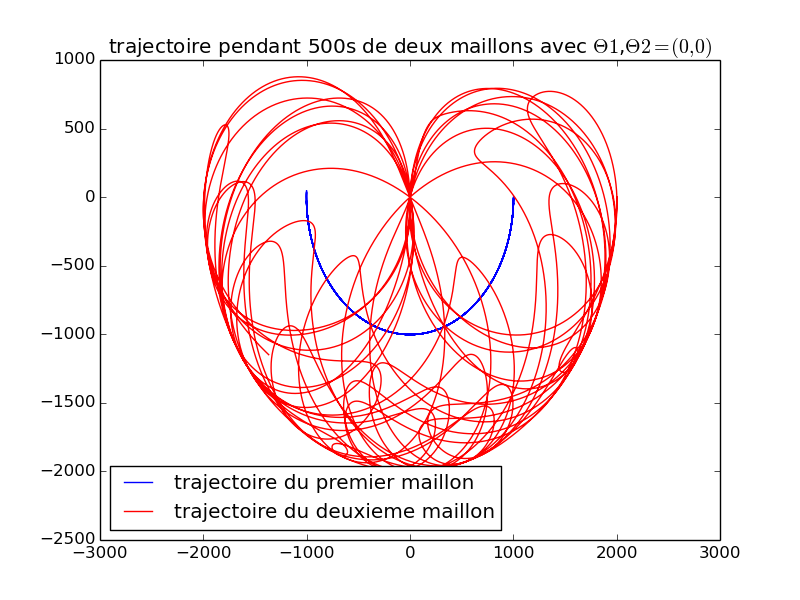
\includegraphics[scale=0.29]{images/deux_maillon.png}   &
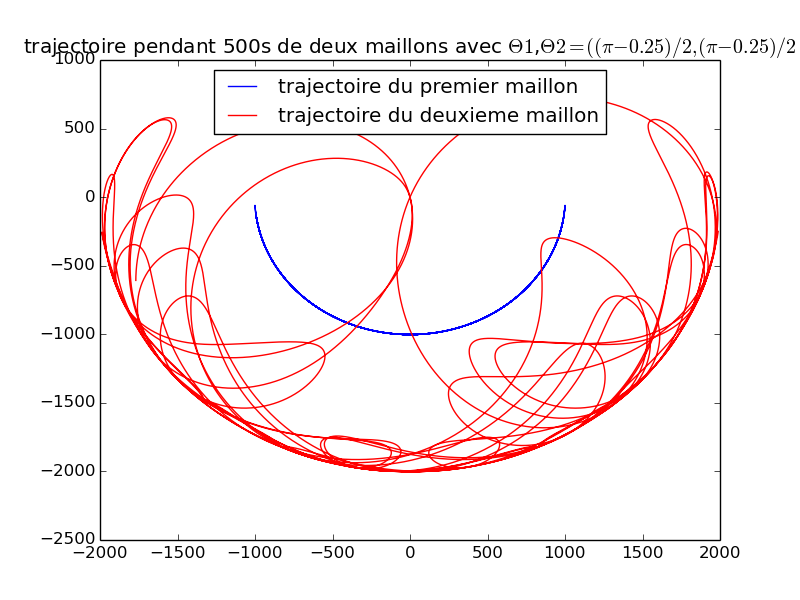
\includegraphics[scale=0.29]{images/deux_maillon_1.png} &
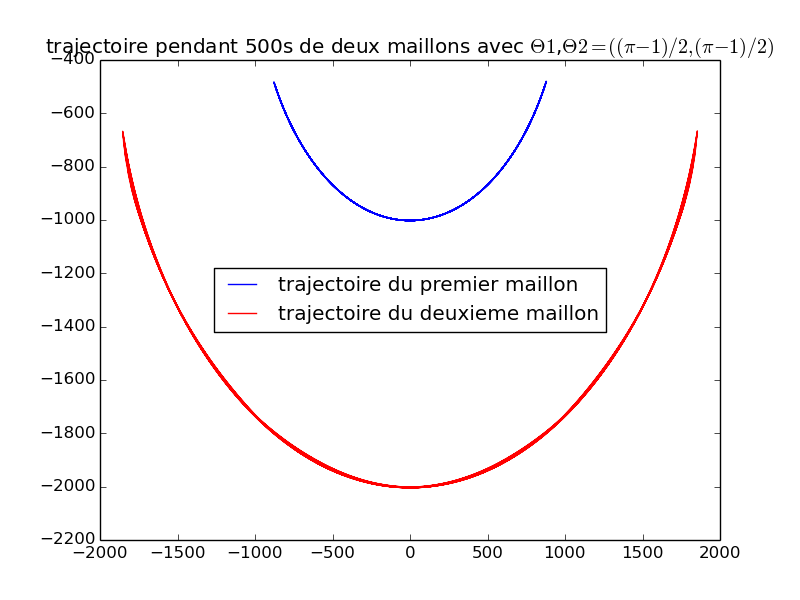
\includegraphics[scale=0.29]{images/deux_maillon_2.png} 
\end{tabular}
\caption{Comparaison des trajectoires du pendules par rapport à $\theta_1$,$\theta_2$}
\label{Fig:3}
\end{figure}
Enfin, une autre façon de mettre en valeur le caractère chaotique du système consistait à déterminer le temps du premier retournement. Cela signifie d'enregistrer le temps que prends le deuxième maillon avant de dépasser soit $-\pi$ ou $\pi$ selon le signe de $\omega_2$.\\
Le graphe obtenue (Figure \ref{Fig:4}) a plusieurs propriétés. On remarque d’abord que le partie est blanche est celle ou le pendule n'a pas de renversement et que celle-ci est symétrique par rapport au point ($0$,$0$). Cela peut être justifier par la symétrie des fonctions cosinus et sinus.\\
On remarque aussi que le système devient moins chaotique lorsqu'on s'approche du point (0,0) et qu'on peut avoir des résultats très différents lorsqu'on s’éloigne du point ($0$,$0$) en changeant légèrement les conditions initiales.
\begin{figure}[h]
\centering
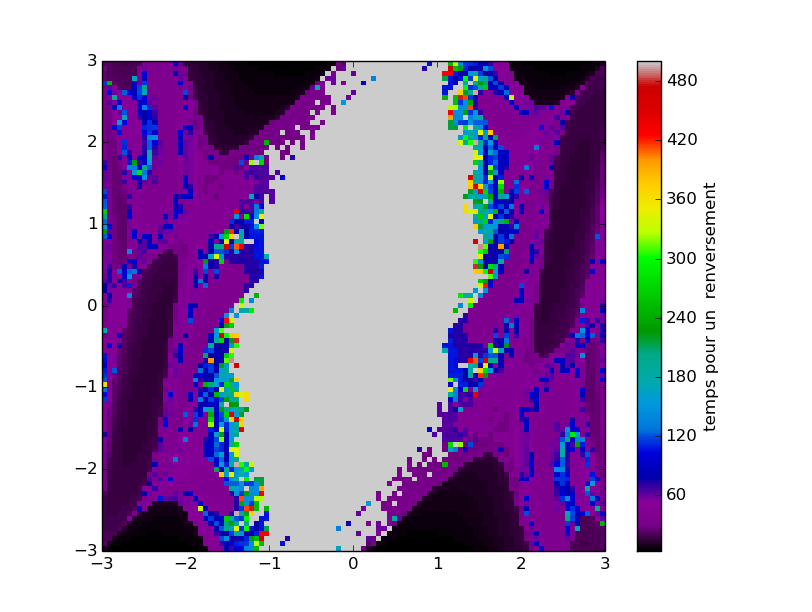
\includegraphics[scale=0.5]{images/map_renversement.png}
\caption{graphe représentant le temps de retournement en fonction de ($\theta_1,\theta_2$)}
\label{Fig:4}
\end{figure}
\end{document}

	